

\Large{The Experiment}
%TODO Get rid of 4panel, put the top left picture, include text/caption explaining the setting based on picture added
\normalsize
\begin{figure}
\begin {center}
\begin {tikzpicture}[-latex ,auto ,node distance =3cm and 4cm ,on grid ,
semithick ,
state/.style ={ circle ,top color =white , bottom color = processblue!20 ,
draw,processblue , text=blue , minimum width =1 cm}]
\node[state] (C){$Sold$};
\node[state] (A) [above left=of C] {$Recession$};
\node[state] (B) [above right =of C] {$Booming$};
\coordinate[below left of=C] (D);
\coordinate[below right of=C] (E);

\path (A) edge [loop left] node[left] {$0.86$} (A);
\path (A) edge [bend left = -25] node[below =0.25 cm] {$1$} (C);
\path (A) edge [bend left =25] node[above] {$0.14$} (B);

\path (B) edge [loop right] node[right] {1} (B);
\path (B) edge [bend right = -25] node[below =0.25 cm] {$1$} (C);

%\fill[gray!40!white, opacity=0.5] (-6,-1) rectangle (5,6);
\pause
\path (A) edge [bend right =25] node[left] {$Observation$} (D);
\path (B) edge [bend left =25] node[right] {$Observation$} (E);
\end{tikzpicture}
\end{center}
\end{figure}

\begin{itemize}
    \item In a simulated housing market, participants needed to decide whether to sell or to wait.
    \item Waiting decreases risk, but increases costs.
    \item 24 participants performed three different scenarios.
\end{itemize}

\begin{figure}
  \centering
    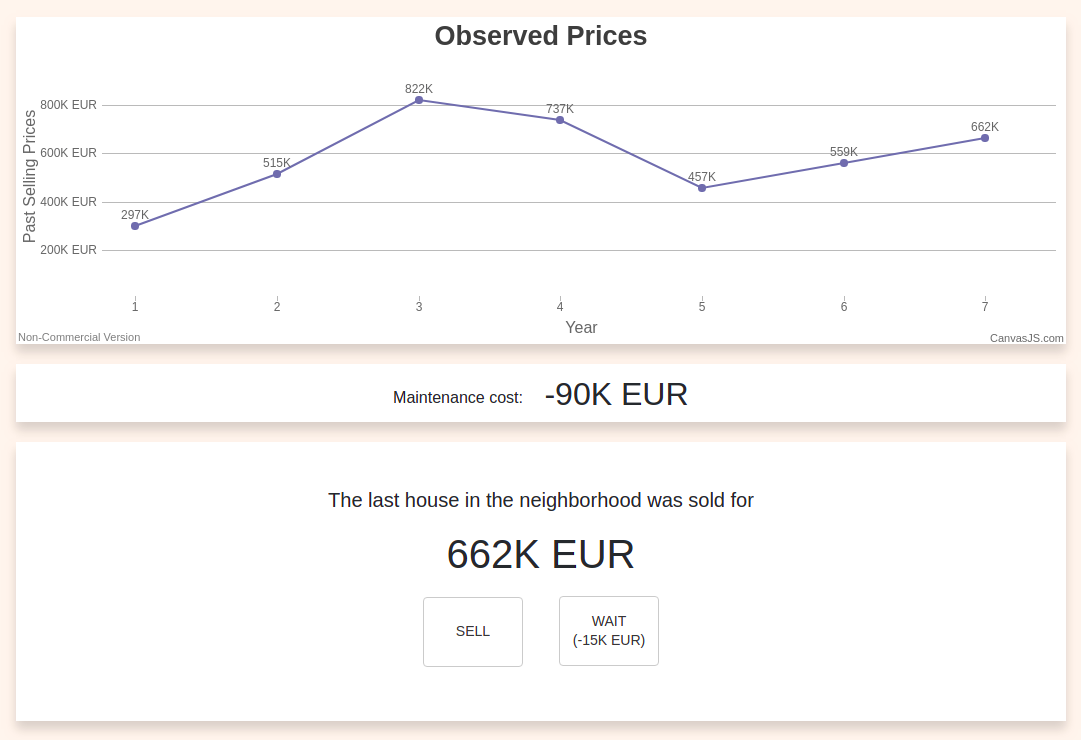
\includegraphics[width=0.9\textwidth]{img/methods/experiment_obs_1.png}
  \caption{Part of the UI used in the experiment showing the observation history.}
\end{figure}


\Large{The Agent}
\normalsize
\begin{itemize}
    \item Simplify POMDP into a MDP by Bayesian estimates.
    \begin{figure}
        \centering
        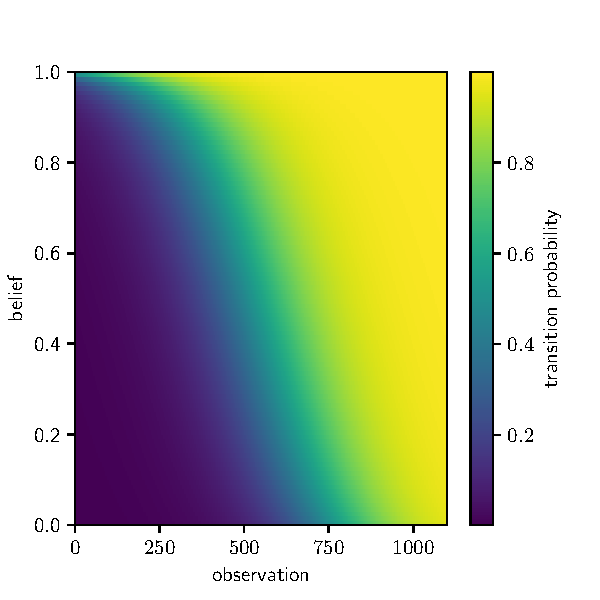
\includegraphics{img/belief_table.pdf}
        \caption{Caption}
        \label{fig:my_label}
    \end{figure}
    \item Solve the MDP with value iteration on an augmented state space.
    % TODO formula for value iteration, expected values separated if it doesn't fit
    \[V^{(n-1)}(b,w) =\ldots\]
    \[Q^{(n)}_{U} (b, w) = \max(\int_{-\inf}^{\inf}{P(o|b)}) \]
    \item Different utility functions.
    % formulas for different utility functions.
\end{itemize}
